\documentclass{article}
\usepackage{url}
\usepackage{graphicx}
\usepackage{float}
\usepackage{biblatex}
\addbibresource{ref.bib}
\graphicspath{{./images}}
\title{Analysis of Sample3.dll \\Practical Assignment 3\\Malware Reverse Engineering \\
CAP6137}
\author{Michael Ivanov \\
ivanovmichael@ufl.edu}
\date{March 14, 2022}
\hfuzz=30pt

\begin{document}
    \maketitle
    \pagebreak
    \section{Executive Summary}
    This malware belongs to the \textit{Emotet} family, a banking Trojan\cite{emotet}. Analysis was challenging due to the large amount of obfuscation. Static analysis provided shows us some anti-debugging techniques to watch out for later. I found 5 different entry points using \textit{IDA Pro}, 3 of them were duplicates and had no interesting code. I focused most of my attention on the \textit{DllEntryPoint} as it was the most interesting. Obfuscation included indirect calls and large amounts of data manipulation.

    Using dynamic analysis I was able to de-obfuscate many library functions used and resolved any functions called with \textit{GetProcAddress}. Because of the numerous calls to \textit{VirtualAlloc} I decided to dump the memory and was able to find a DLL. Looking online this appears to be a common behavior for an \textit{Emotet} family malware. Due to time constraints, I was not able to analyze this dll, but I provided the hashes below. The malware communicates over the network using HTTP/HTTPS traffic.
    \pagebreak
    \section{Static Analysis}
    \subsection{MD5 Hashes}
    \begin{itemize}
        \item sample3.dll: 3AC8BFD8DA5D3C4789D1F5D26E0E082B
        \item unknown resource: 30245F444D61C3C8780A7058381E140A
        \item Virtual allocate dump: D1B9580B68E7A5E5E6792FC5AAF0E593
        \item Virtual allocate dump 2: 481B91ABB4C17C830A779D1302794CD8
    \end{itemize}
    \subsection{Compilation date}
    \begin{itemize}
        \item Sample3.dll: Fri Mar 04, 07:51:31 2022
    \end{itemize}
    \subsection{Suspicious Imports}
    One thing to note is that according to Pestudio, 44 imports are referenced by ordinal.
    \begin{itemize}
        \item \textbf{RegCreateKeyA, RegDeleteValueA, RegSetValueA, RegDeleteKeyA}: these are indicators the malware will probably be modifying the registry.
        \item \textbf{FindFirstFileA, UnlockFile, LockFile, DeleteFileA, MoveFileA}: various file operations
        \item \textbf{GetAtomNameA, GlobalGetAtomNameA, GlobalFindAtomA, GlobalAddAtomA, GlobalDeleteAtom}: Possible dynamic data exchange, which allows for different processes to communicate with each other. \cite{atom}
        \item \textbf{RegisterClipboardFormatA,} \textbf{OleSetClipboardFormatA,} \textbf{OleFlushClipboard}: various clipboard operations.
    \end{itemize}
    \subsection{Suspicious strings}
    The following strings start with \url{f:\dd\vctools\vc7libs\ship\atlmfc\src\mfc\}
    \begin{itemize}
        \item \url{dockcont.cpp}, \url{filecore.cpp}, \url{winctrl2.cpp}, \url{appcore.cpp}, \url{aucdata.cpp}, \url{olefact.cpp}, \url{olestrm.cpp}
    \end{itemize}
    The following strings start with \url{f:\dd\vctools\vc7libs\ship\atlmfc\include\}
    \begin{itemize}
        \item \url{afxwin1.inl}, \url{afxwin2.inl}
    \end{itemize}
    Potential format strings for shell commands:
    \begin{itemize}
        \item \url{%s\shell\open\%s}
        \item \url{%s\shell\print\%s}
        \item \url{%s\shell\printto\%s}
        \item \url{%s\ShellNew}
    \end{itemize}
    A format string for a dll file:
    \begin{itemize}
        \item \url{%s%s.dll}
    \end{itemize}
    \subsection{Program Sections}
    In the resource section (\url{.rsrc}) there is an unknown file. I've provided the hash above. The file seems to be encoded.
    \subsection{Exports}
    \begin{figure}[H]
        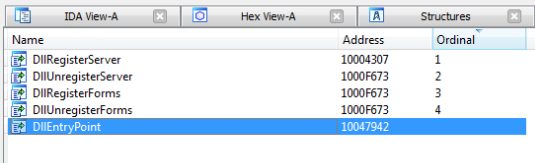
\includegraphics[width=\textwidth]{dllentrypoints.png}
        \caption{List of all exports for sample3.dll using \textit{Ida Pro}}
    \end{figure}
    Using Ghidra I was able to determine that ordinal 1 entry point \textit{DLLRegisterServer} was the most interesting out of the ordinals. The rest were duplicates of each other and did not do anything. However the entry point \textit{DLLEntryPoint} was the most interesting, and most of the report will be focused on analyzing this entry point.
    \begin{figure}[H]
        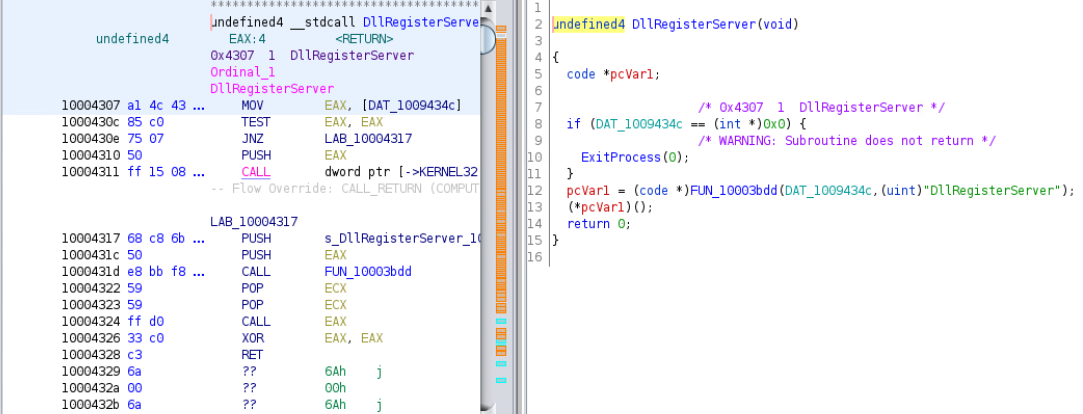
\includegraphics[width=\textwidth]{export1.png}
        \caption{Ordinal 1 entry point \textit{DLLRegisterServer}}
    \end{figure}
    \begin{figure}[H]
        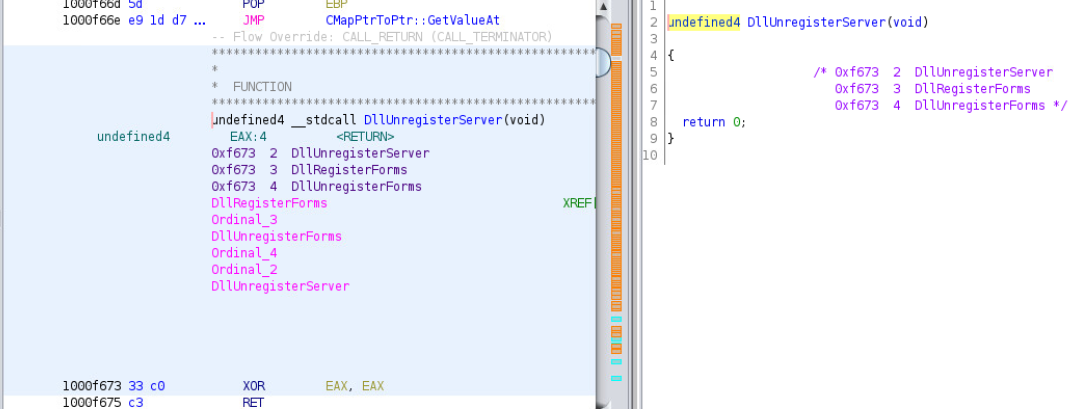
\includegraphics[width=\textwidth]{exports2-4.png}
        \caption{Ordinals 2-4 empty entry points}
    \end{figure}
    \subsection{Anti-disassembly}
    I was not able to find any signs of anti-disassembly.
    \subsection{Anti-debugging}
    \begin{figure}[H]
        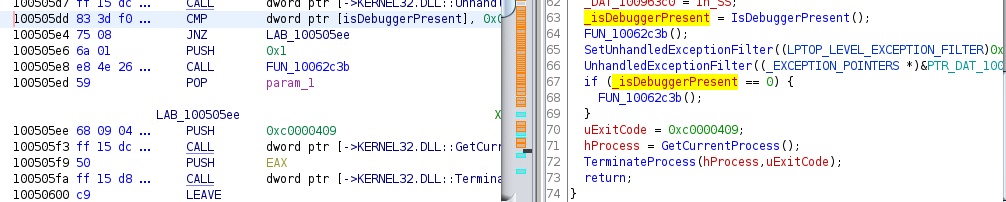
\includegraphics[width=\textwidth]{antidebuging.png}
        \caption{A check in a function at the end of DLLMain for debugging}
    \end{figure}
    \subsection{Obfuscation}
    Below is an indirect call inside the ordinal 1 entry point. The function above returns the address to the call.
    \begin{figure}[H]
        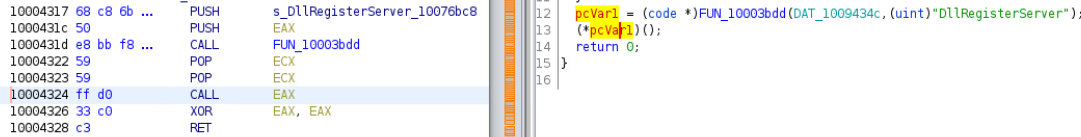
\includegraphics[width=\textwidth]{ord1obf.png}
        \caption{Ordinal 1 entry disassembly of an indirect call}
    \end{figure}
    In the \textit{DLLEntryPoint} there are numerous examples of obfuscation of data. Below is an example found in DLLMain:
    \begin{figure}[H]
        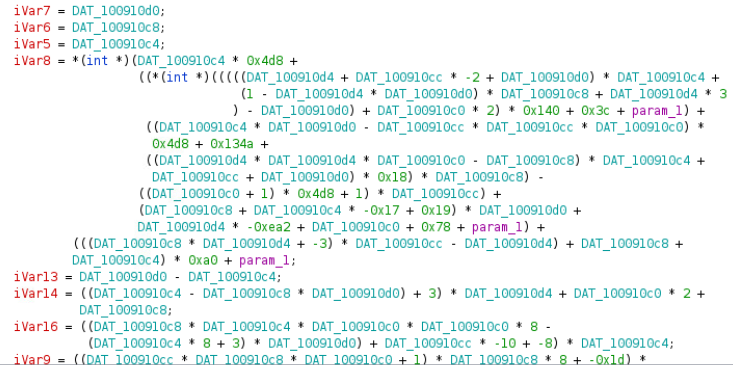
\includegraphics[width=\textwidth]{obfex.png}
        \caption{Example of obfuscation in DLLMain}
    \end{figure}
    \pagebreak
    \section{Dynamic Analysis}
    \subsection{Interesting behaviors}
    This malware has lots of deobfuscation, making static analysis challenging. The malware uses a few different anti-debugging techniques as discussed below. I was able to make a pop-up screen to appear by manually changing a control flow bit in x32dbg to continue executing a function.

    By dumping the memory after a call to VirtualAlloc I was able to extract a Dll. I provided the hash above.
    \begin{figure}[H]
        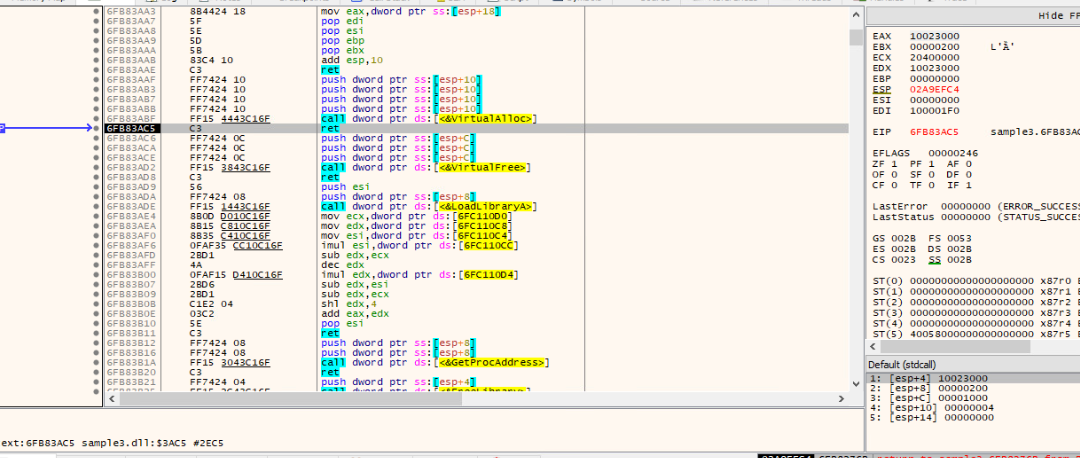
\includegraphics[width=\textwidth]{virtalloc.png}
        \caption{The call to VirtualAlloc at RVA 3ABF}
    \end{figure}
    By using the value in EDX I was able to dump the memory into a file:
    \begin{figure}[H]
        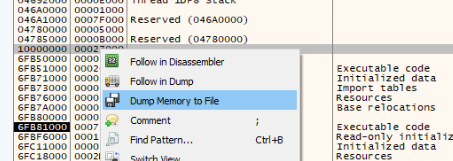
\includegraphics[width=\textwidth]{dump.png}
        \caption{Extracting the memory to a file}
    \end{figure}
    \begin{figure}[H]
        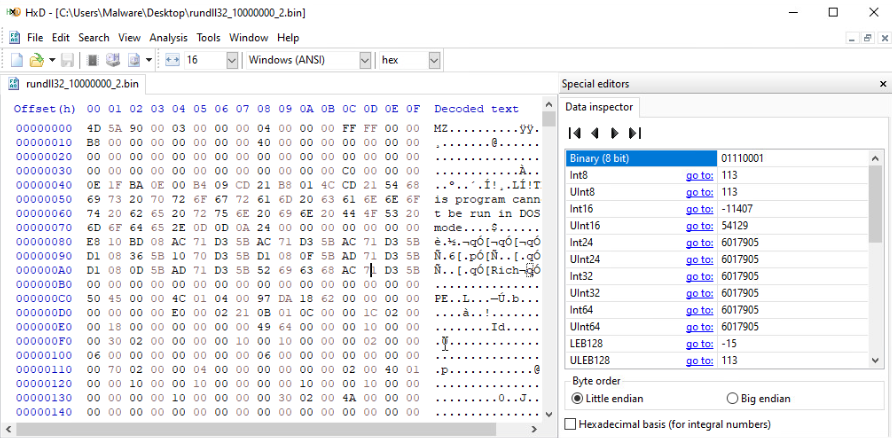
\includegraphics[width=\textwidth]{hxdump.png}
        \caption{A quick look at the binary}
    \end{figure}
    \subsection{Networking activity}
    The following are network traffic found by running sample3.dll on ordinal 1:
    \begin{itemize}
        \item 51.75.33.122:https
        \item 186.250.45.5:http
        \item 168.119.39.118:https
        \item 85.214.67.203:8080
    \end{itemize}
    \begin{figure}[H]
        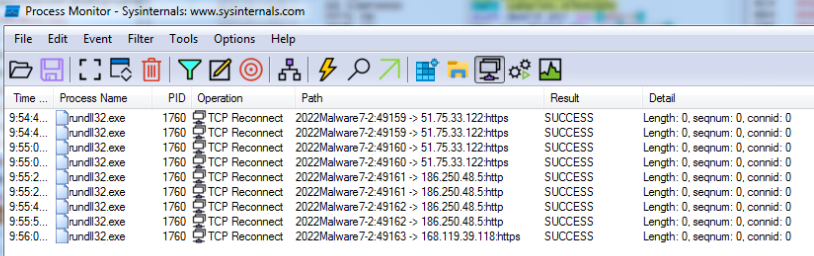
\includegraphics[width=\textwidth]{networkProcmon.png}
        \caption{Example network activity shown by \textit{Procmon}}
    \end{figure}
    \subsection{Registry keys created or modified}
    Registry keys modified:
    \begin{itemize}
        \item \url{HKCU\Software\Microsoft\Windows\CurrentVersion\Internet Settings\Connections\SavedLegacySettings}
        \item \url{HKCU\Software\Microsoft\Windows\CurrentVersion\Internet Settings\ZoneMap\ProxyBypass}
        \item \url{HKCU\Software\Microsoft\Windows\CurrentVersion\Internet Settings\ProxyEnable}
        \item \url{HKCU\Software\Microsoft\Windows\CurrentVersion\Internet Settings\ZoneMap\UNCAsIntranet}
        \item \url{HKCU\Software\Microsoft\Windows\CurrentVersion\Internet Settings\ZoneMap\AutoDetect}
        \item \url{HKCU\Software\Microsoft\Windows\CurrentVersion\Internet Settings\ZoneMap\IntranetName}
        \item \url{HKCU\Software\Microsoft\Windows\CurrentVersion\Internet Settings\Wpad\00-50-56-87-c7-d5\WpadDecisionReason}
        \item \url{HKCU\Software\Microsoft\Windows\CurrentVersion\Internet Settings\Wpad\00-50-56-87-c7-d5\WpadDecisionTime}
        \item \url{HKCU\Software\Microsoft\Windows\CurrentVersion\Internet Settings\Wpad\00-50-56-87-c7-d5\WpadDecision}
        \item \url{HKCU\Software\Microsoft\Windows\CurrentVersion\Internet Settings\Wpad\00-50-56-87-c7-d5\WpadDetectedUrl}
        \item \url{HKCU\Software\Microsoft\Windows\CurrentVersion\Internet Settings\Wpad\{082A014B-1185-406F-8FE4-BB152F2E1081}\WpadDecisionReson}
        \item \url{HKCU\Software\Microsoft\Windows\CurrentVersion\Internet Settings\Wpad\{082A014B-1185-406F-8FE4-BB152F2E1081}\WpadDecisionTime}
        \item \url{HKCU\Software\Microsoft\Windows\CurrentVersion\Internet Settings\Wpad\{082A014B-1185-406F-8FE4-BB152F2E1081}\WpadDecision}
        \item \url{HKCU\Software\Microsoft\Windows\CurrentVersion\Internet Settings\Wpad\{082A014B-1185-406F-8FE4-BB152F2E1081}\WpadNetworkName}
    \end{itemize}
    \begin{figure}[H]
        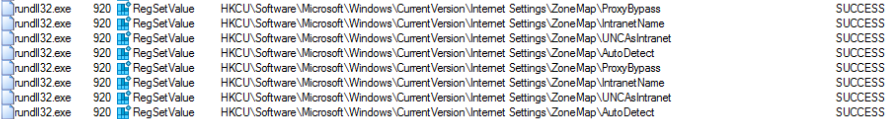
\includegraphics[width=\textwidth]{regkeyset.png}
        \caption{Example registry key activity shown by \textit{Procmon}}
    \end{figure}
    \subsection{Functions found through debugging}
    Functions found by tracing \url{eip < addr1 || eip >= addr2}
    Where addr1 and addr2 are the bounds to the program text section.
    \begin{itemize}
        \item Function Name: RVA
        \item HeapCreate
        \item GetModuleHandleW: 50297, 4FE05
        \item FlsAlloc: 502BE
        \item FlsGetValue: 502CB
        \item FlsSetValue: 502D8
        \item FlsFree: 502E5
        \item TlsAlloc: 50335
        \item TlsSetValue: 50350
        \item TlsGetValue: 4fDD8
        \item EncodePointer: 4FE20
        \item ZwQueryInformationProcess: 4FE2D
        \item GetCommandLineA: 4774D
        \item GetEnvironmentStringsW: 5358B
        \item WideCharToMultiByte: 53600
        \item RtlAllocateHeap: 474E6
        \item FreeEnvironmentStringsW: 53639
        \item GetStartupInfoA: 52F9E
        \item GetStdHandle: 53152
        \item SetHandleCount: 531BC
        \item GetLastError: 50055
        \item SetlastError: 500BF
        \item RtlEnterCriticalSection: 509D6
        \item RtlLeaveCriticalSection: 508C9
        \item GetACP: 57E26
    \end{itemize}
    The following are functions resolved from \url{GetProcAddress}:
    \begin{itemize}
        \item FlsAlloc
        \item FlsGetValue
        \item FlsSetValue
        \item FlsFree
        \item EncodePointer
        \item DecodePointer
        \item IsProcessorFeaturePresent
    \end{itemize}
    \begin{figure}[H]
        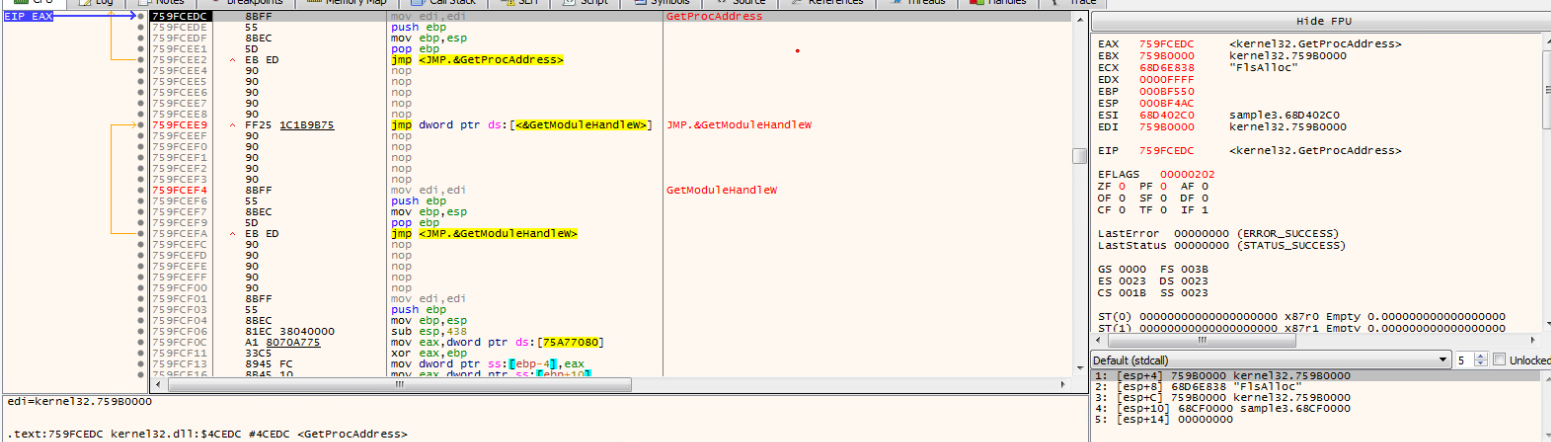
\includegraphics[width=\textwidth]{resolveprocaddress.png}
        \caption{Example function being resolved from \textit{GetProcAddress}}
    \end{figure}
    \subsection{Files created or modified}
    No files were created or modified.
    \subsection{Processes started}
    No processes were started, below are some threads that were created:
    \begin{figure}[H]
        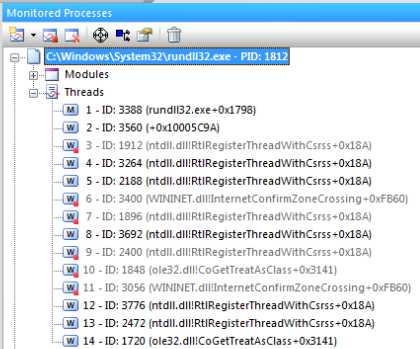
\includegraphics[width=\textwidth]{threads.png}
        \caption{Threads started by \textit{sample3.dll}}
    \end{figure}
    \subsection{Persistence}
    There appears to be no persistence that I could find. Some registry keys are set which persist, but the malware does not to be running on reboot. I tried using volatility on reboot to see any process was un-listed, but I could not find any. Network traffic appears to stop as well.
    \subsection{De-obfuscation}
    Deobfuscation was done mainly by using x32dbg by stepping through. I was able to better understand the program control flow and any library functions used. 
    \subsection{Anti-debugging}
    The program displayed the message box below due calling \textit{UnhandledExceptionFilter}. This function "\textit{passes unhandled exceptions to the debugger, if the process is being debugged. Otherwise, it optionally displays an Application Error message box and causes the exception handler to be executed}"\Cite{unhandledFilter}.
    \begin{figure}[H]
        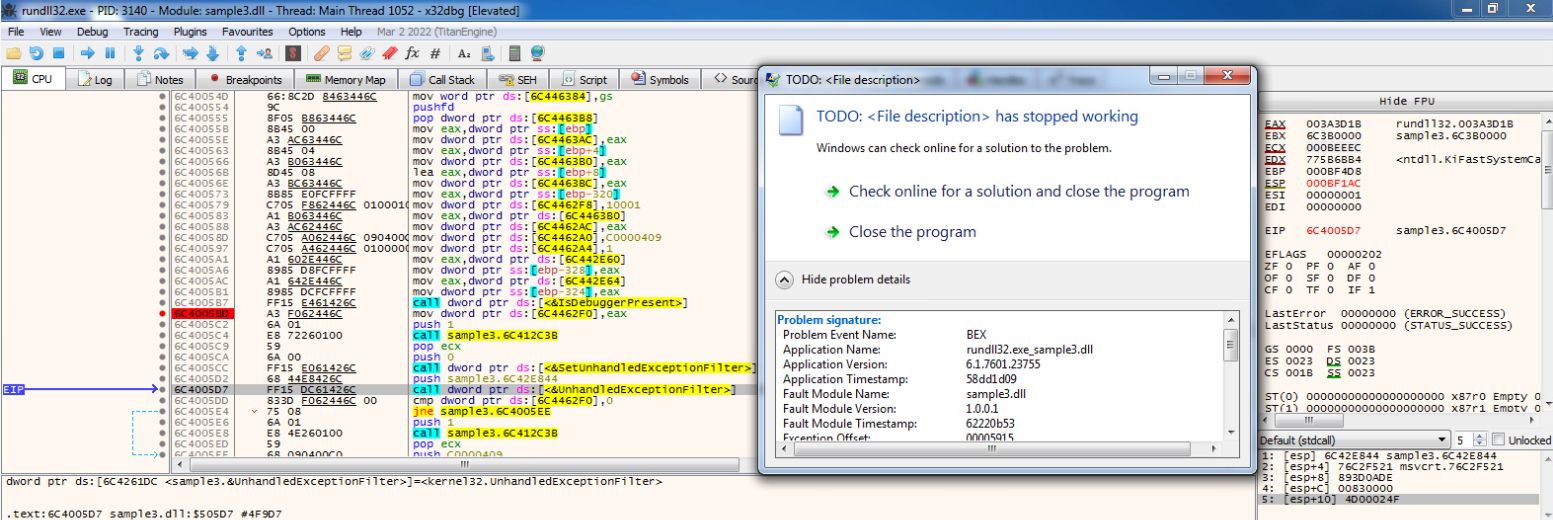
\includegraphics[width=\textwidth]{mesgbox2.png}
        \caption{A message box appearing while debugging}
    \end{figure}
    \pagebreak
    \section{Indicators of Compromise}
    \subsection{Host Indicators}
    \begin{itemize}
        \item sample3.dll: 3AC8BFD8DA5D3C4789D1F5D26E0E082B
    \end{itemize}
    \subsection{Network Indicators}
    Network activity to the following:
    \begin{itemize}
        \item 51.75.33.122:https
        \item 186.250.45.5:http
        \item 168.119.39.118:https
        \item 85.214.67.203:8080
    \end{itemize}
    \subsection{Yara Rule}
    \begin{verbatim}
    import "pe"
    
    rule sample3 {
        meta:
            author = "Michael Ivanov"
        strings:
            $s1 = "olefact.cpp" fullword ascii
            $s2 = "DllRegisterServer" fullword ascii
            $s3 = "DllUnregisterServer" fullword ascii
            $s4 = "DllUnregisterForms" fullword ascii
        condition:
            uint16(0) == 0x5A4D
            and $s1 and $s2 and $s3 and $s4
    }
    \end{verbatim}
    \pagebreak
    \printbibliography
\end{document}